\chapter{Resultados y Experimentación}\label{chapter:implementation}
Después de definir la metodología empleada, se presentan los hallazgos obtenidos durante el estudio de inmunopuente. Primero, se describen los niveles de anticuerpos mediante el cálculo de las medias geométricas de los títulos (GMT) por serotipo según el método empleado. Después, se analizan las razones de medias geométricas (GMR) para evaluar la no inferioridad y, por último, se muestra cómo influyeron los datos censurados en estas estimaciones.

\section{Cálculo de medias geométricas}

Los ensayos clínicos demostraron que, en general, la población adulta tuvo una respuesta opsonofagocítica superior a la de la población pediátrica.

\begin{figure}[ht]
	\centering
	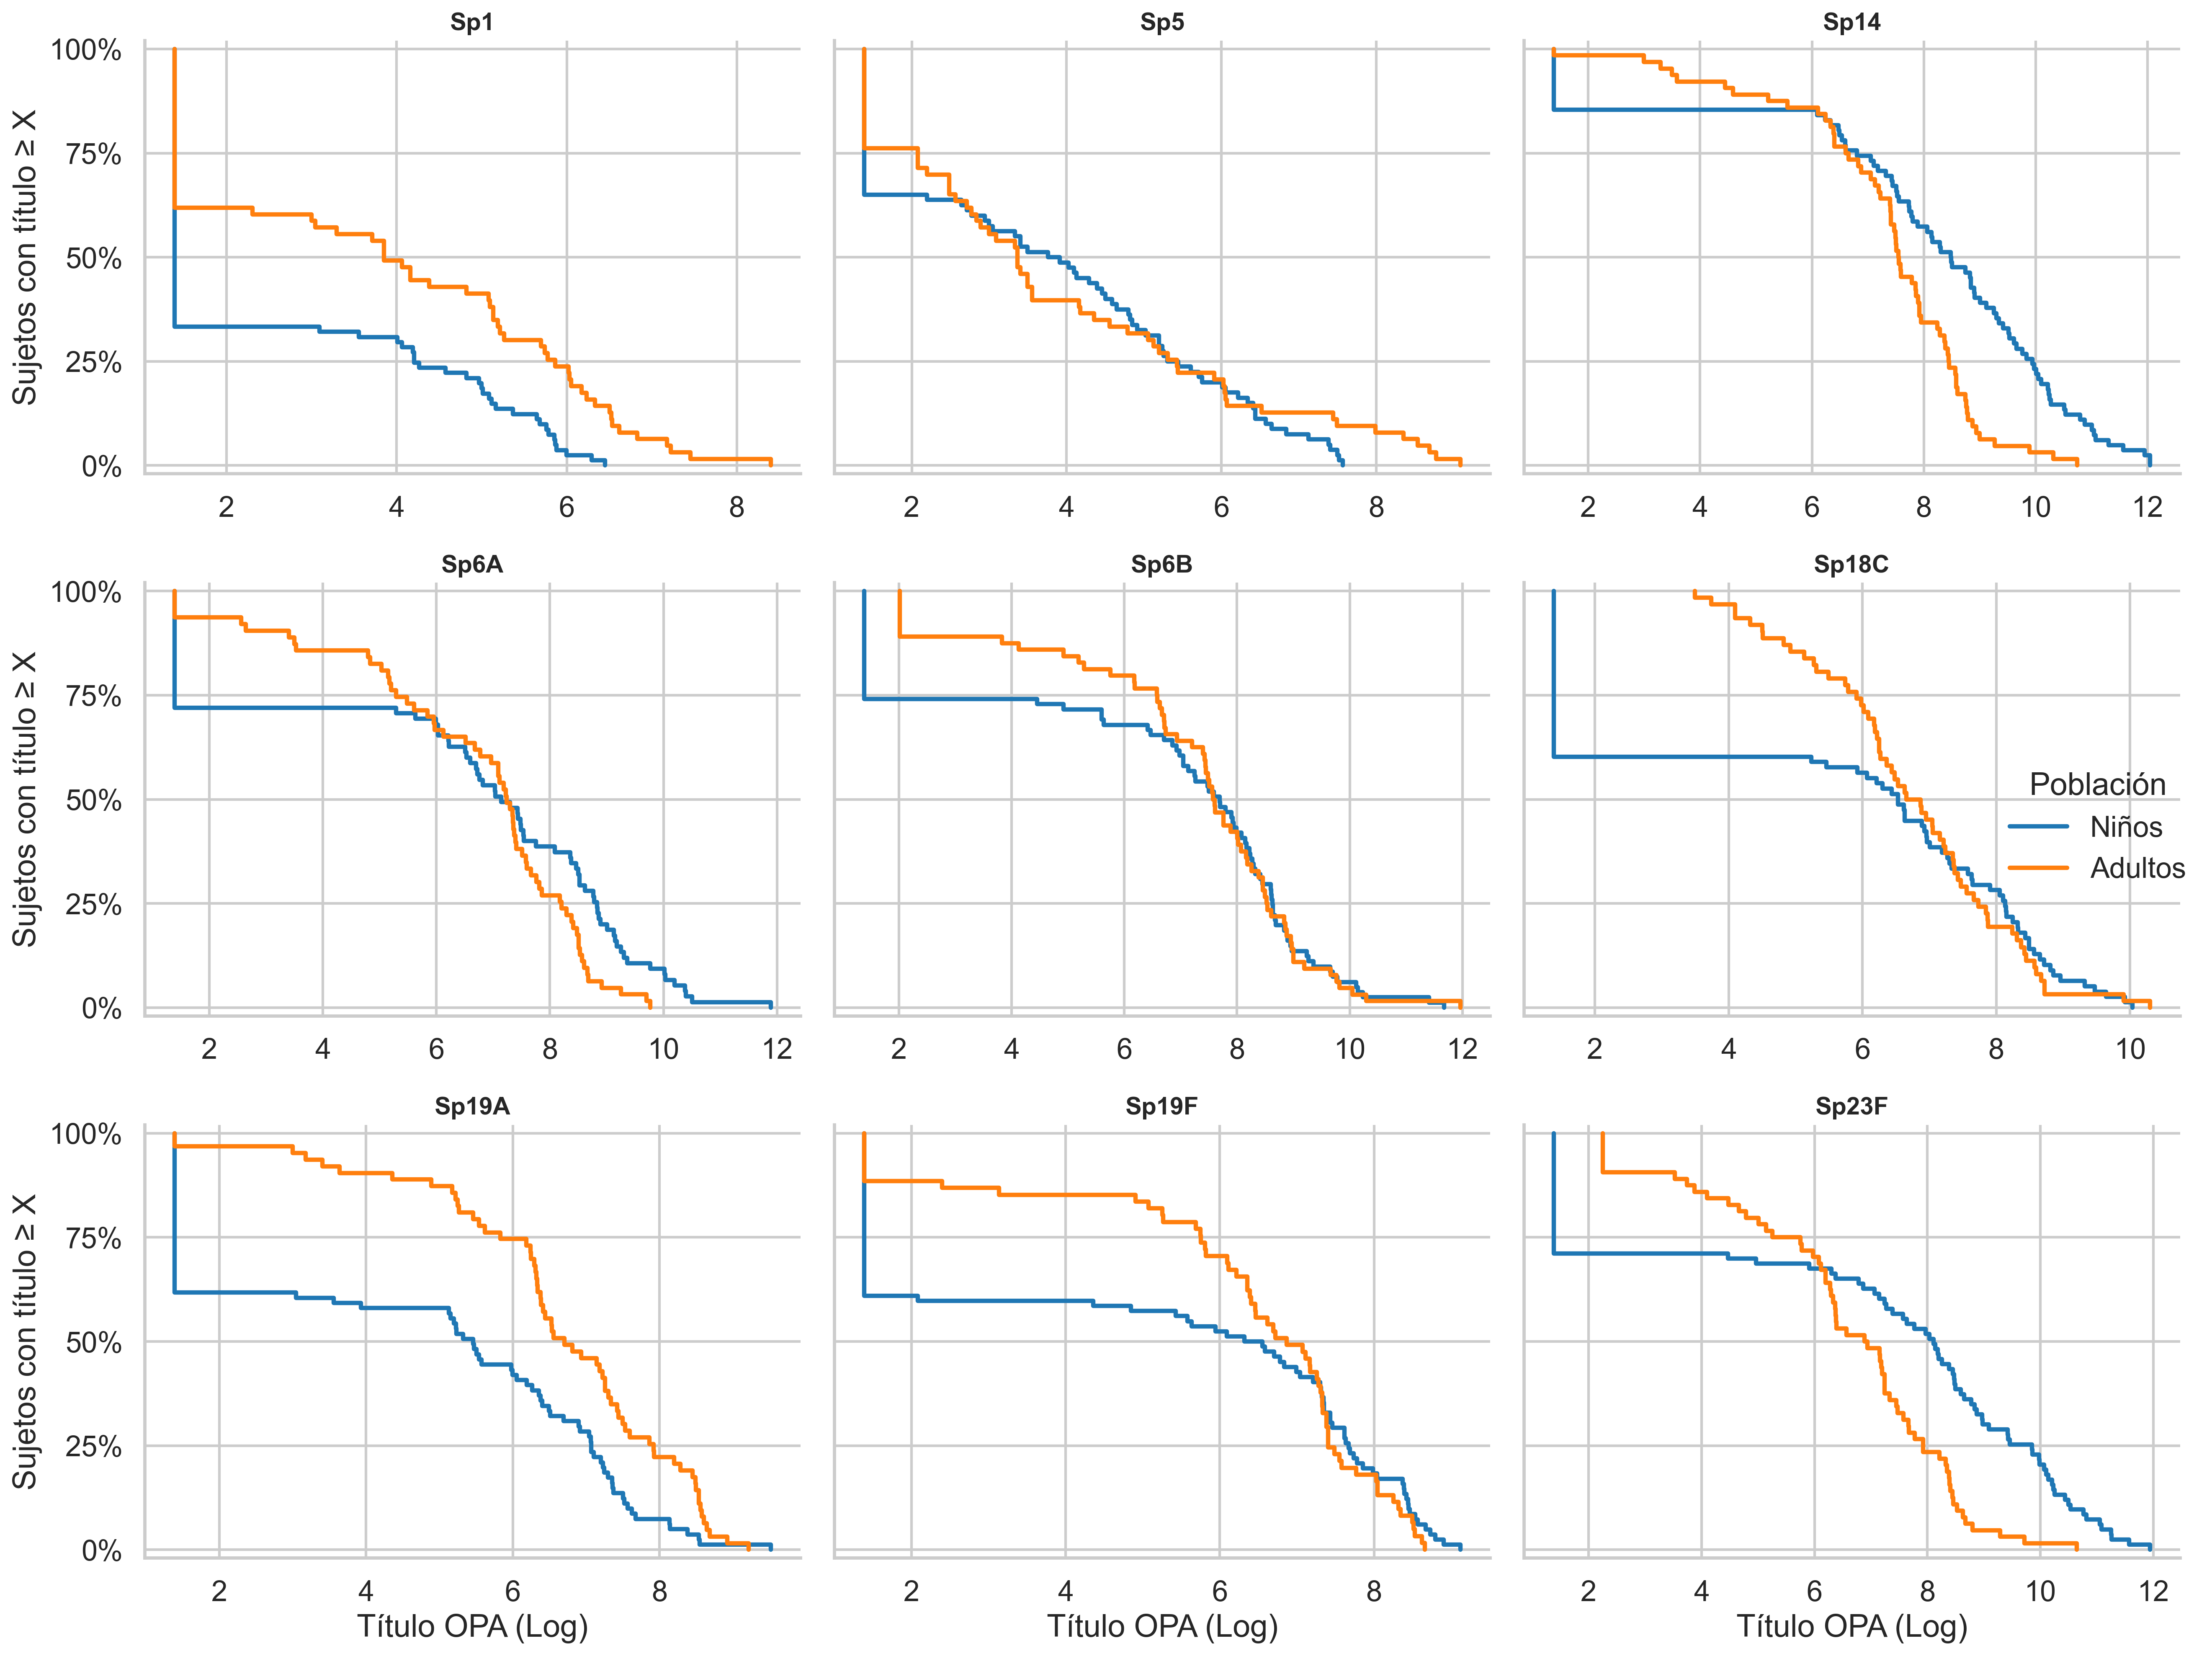
\includegraphics[width=1.0\textwidth]{Graphics/rcdc_results.png}
	\caption{Curvas RCDC por serotipo de los valores OPA de niños y adultos un mes después de la vacunación.}
	\label{fig:rcdc}
\end{figure}
\FloatBarrier

Este patrón se observó al analizar las curvas de distribución de frecuencia acumulativa inversa (Figura \ref{fig:rcdc}), con excepción de los serotipos 14 y 23F que mostraron un comportamiento inverso en los niveles de respuesta más altos.

La diferencia en la distribución de las respuestas también se refleja de manera cuantitativa al calcular las GMT con ambos métodos analíticos (Figuras \ref{fig:gmt_graph1} y \ref{fig:gmt_graph2}).

\begin{figure}[ht]
	\centering
	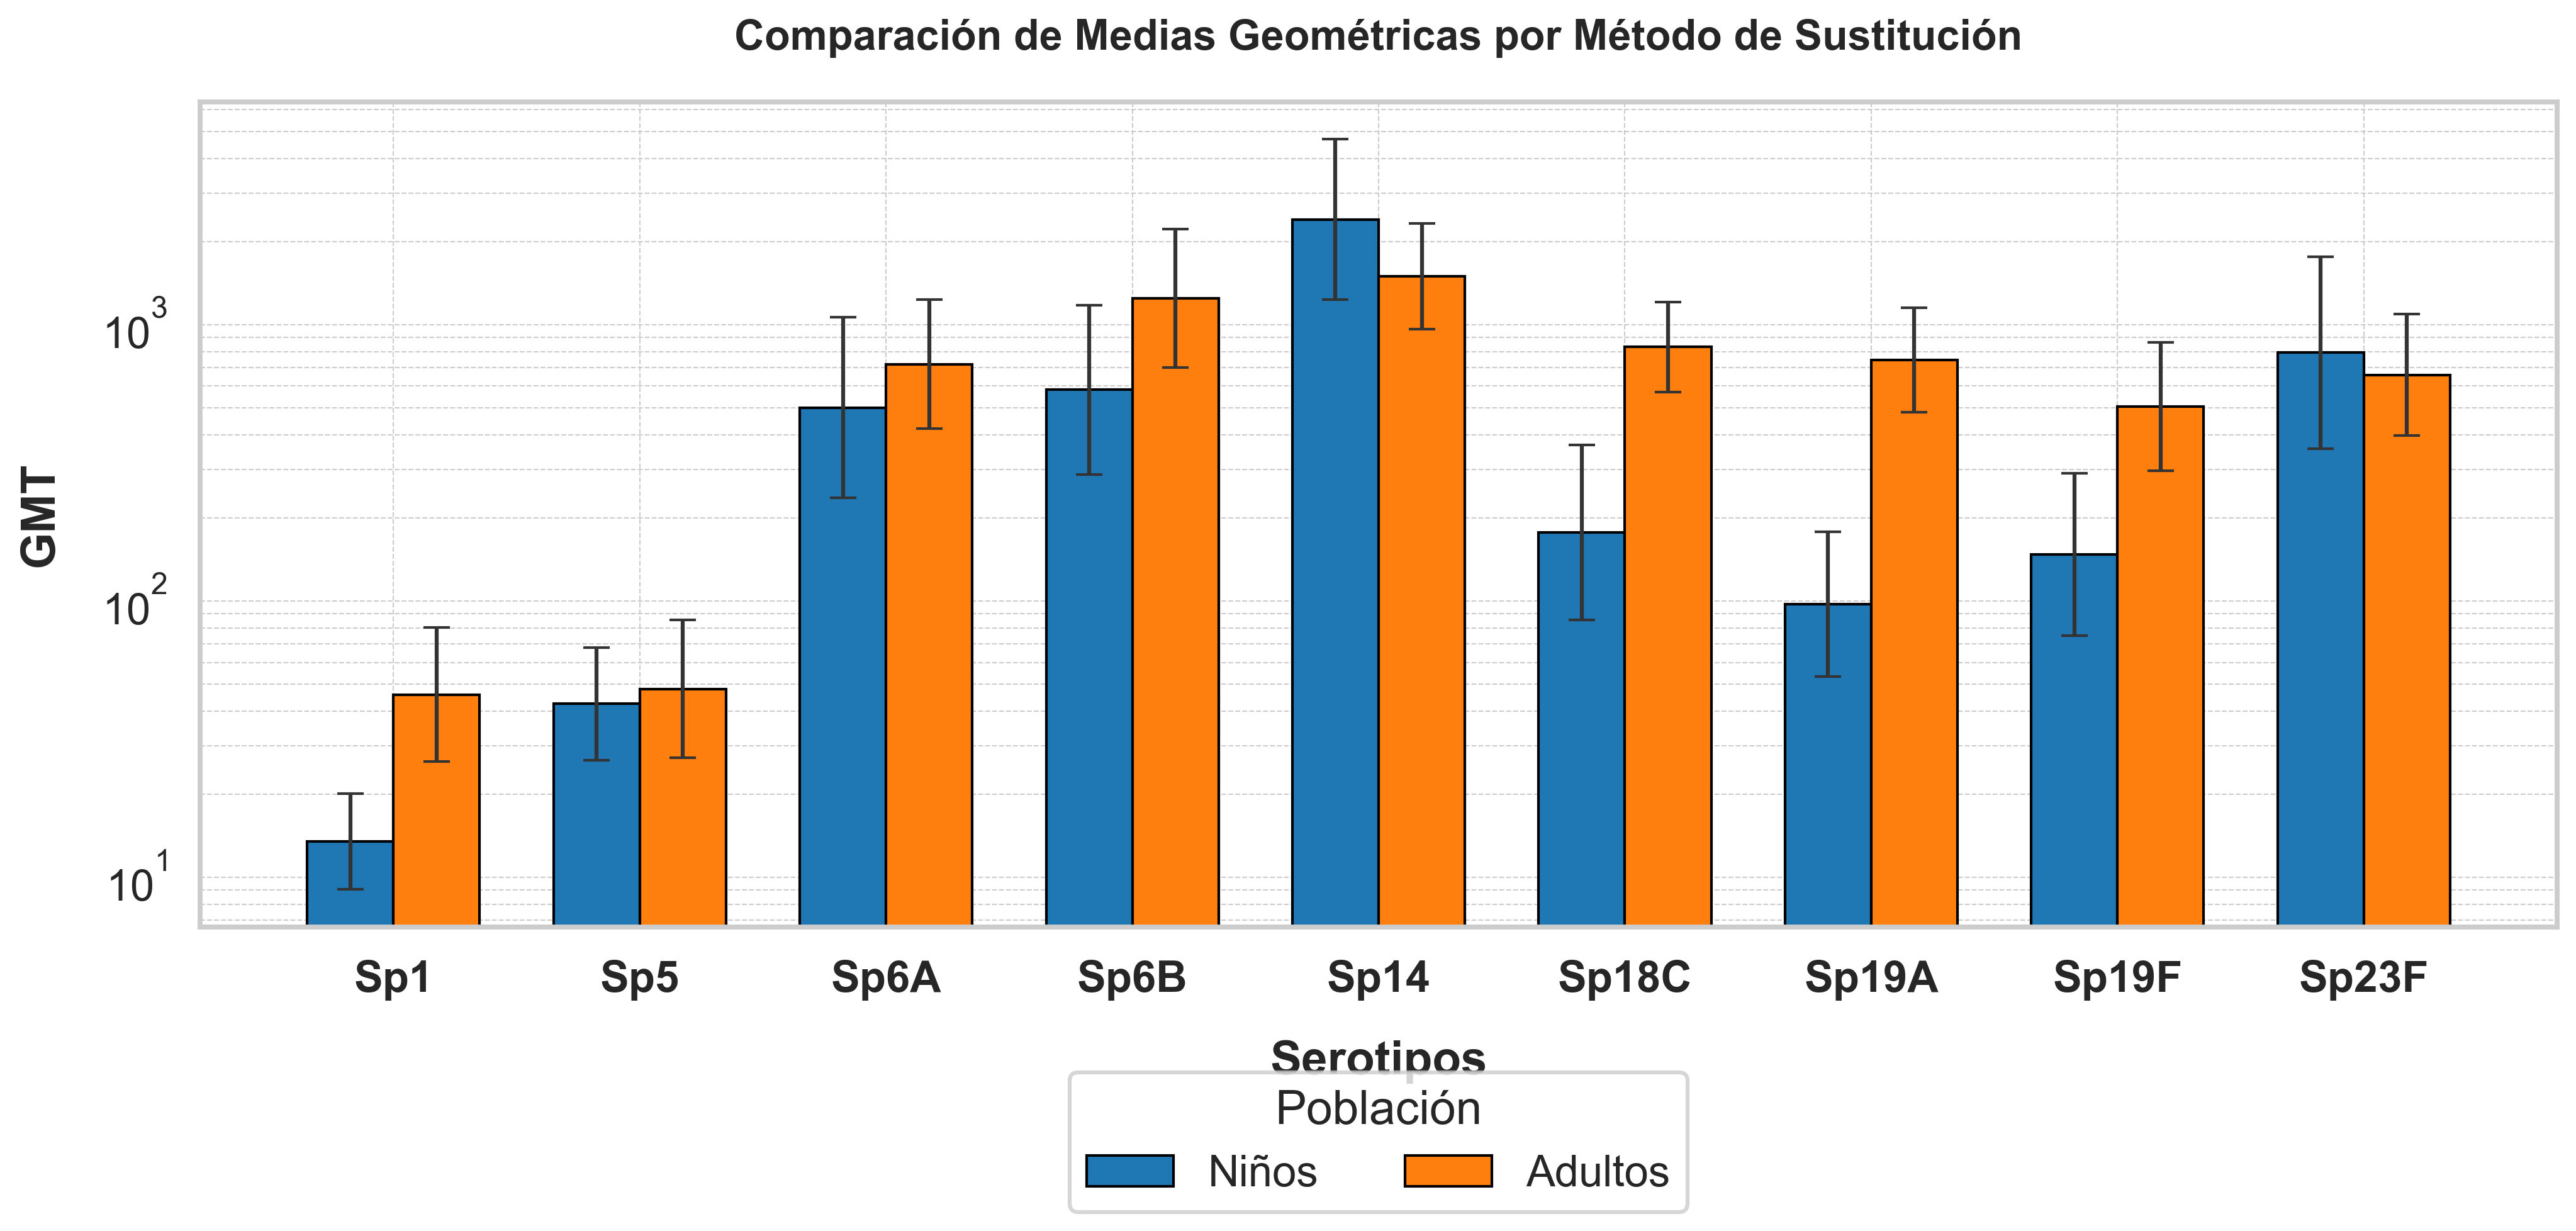
\includegraphics[width=1.0\textwidth]{Graphics/gmts.png}
	\caption{Medias geométricas de los títulos utilizando el método de sustitución.}
	\label{fig:gmt_graph1}
\end{figure}
\FloatBarrier

\begin{figure}[ht]
	\centering
	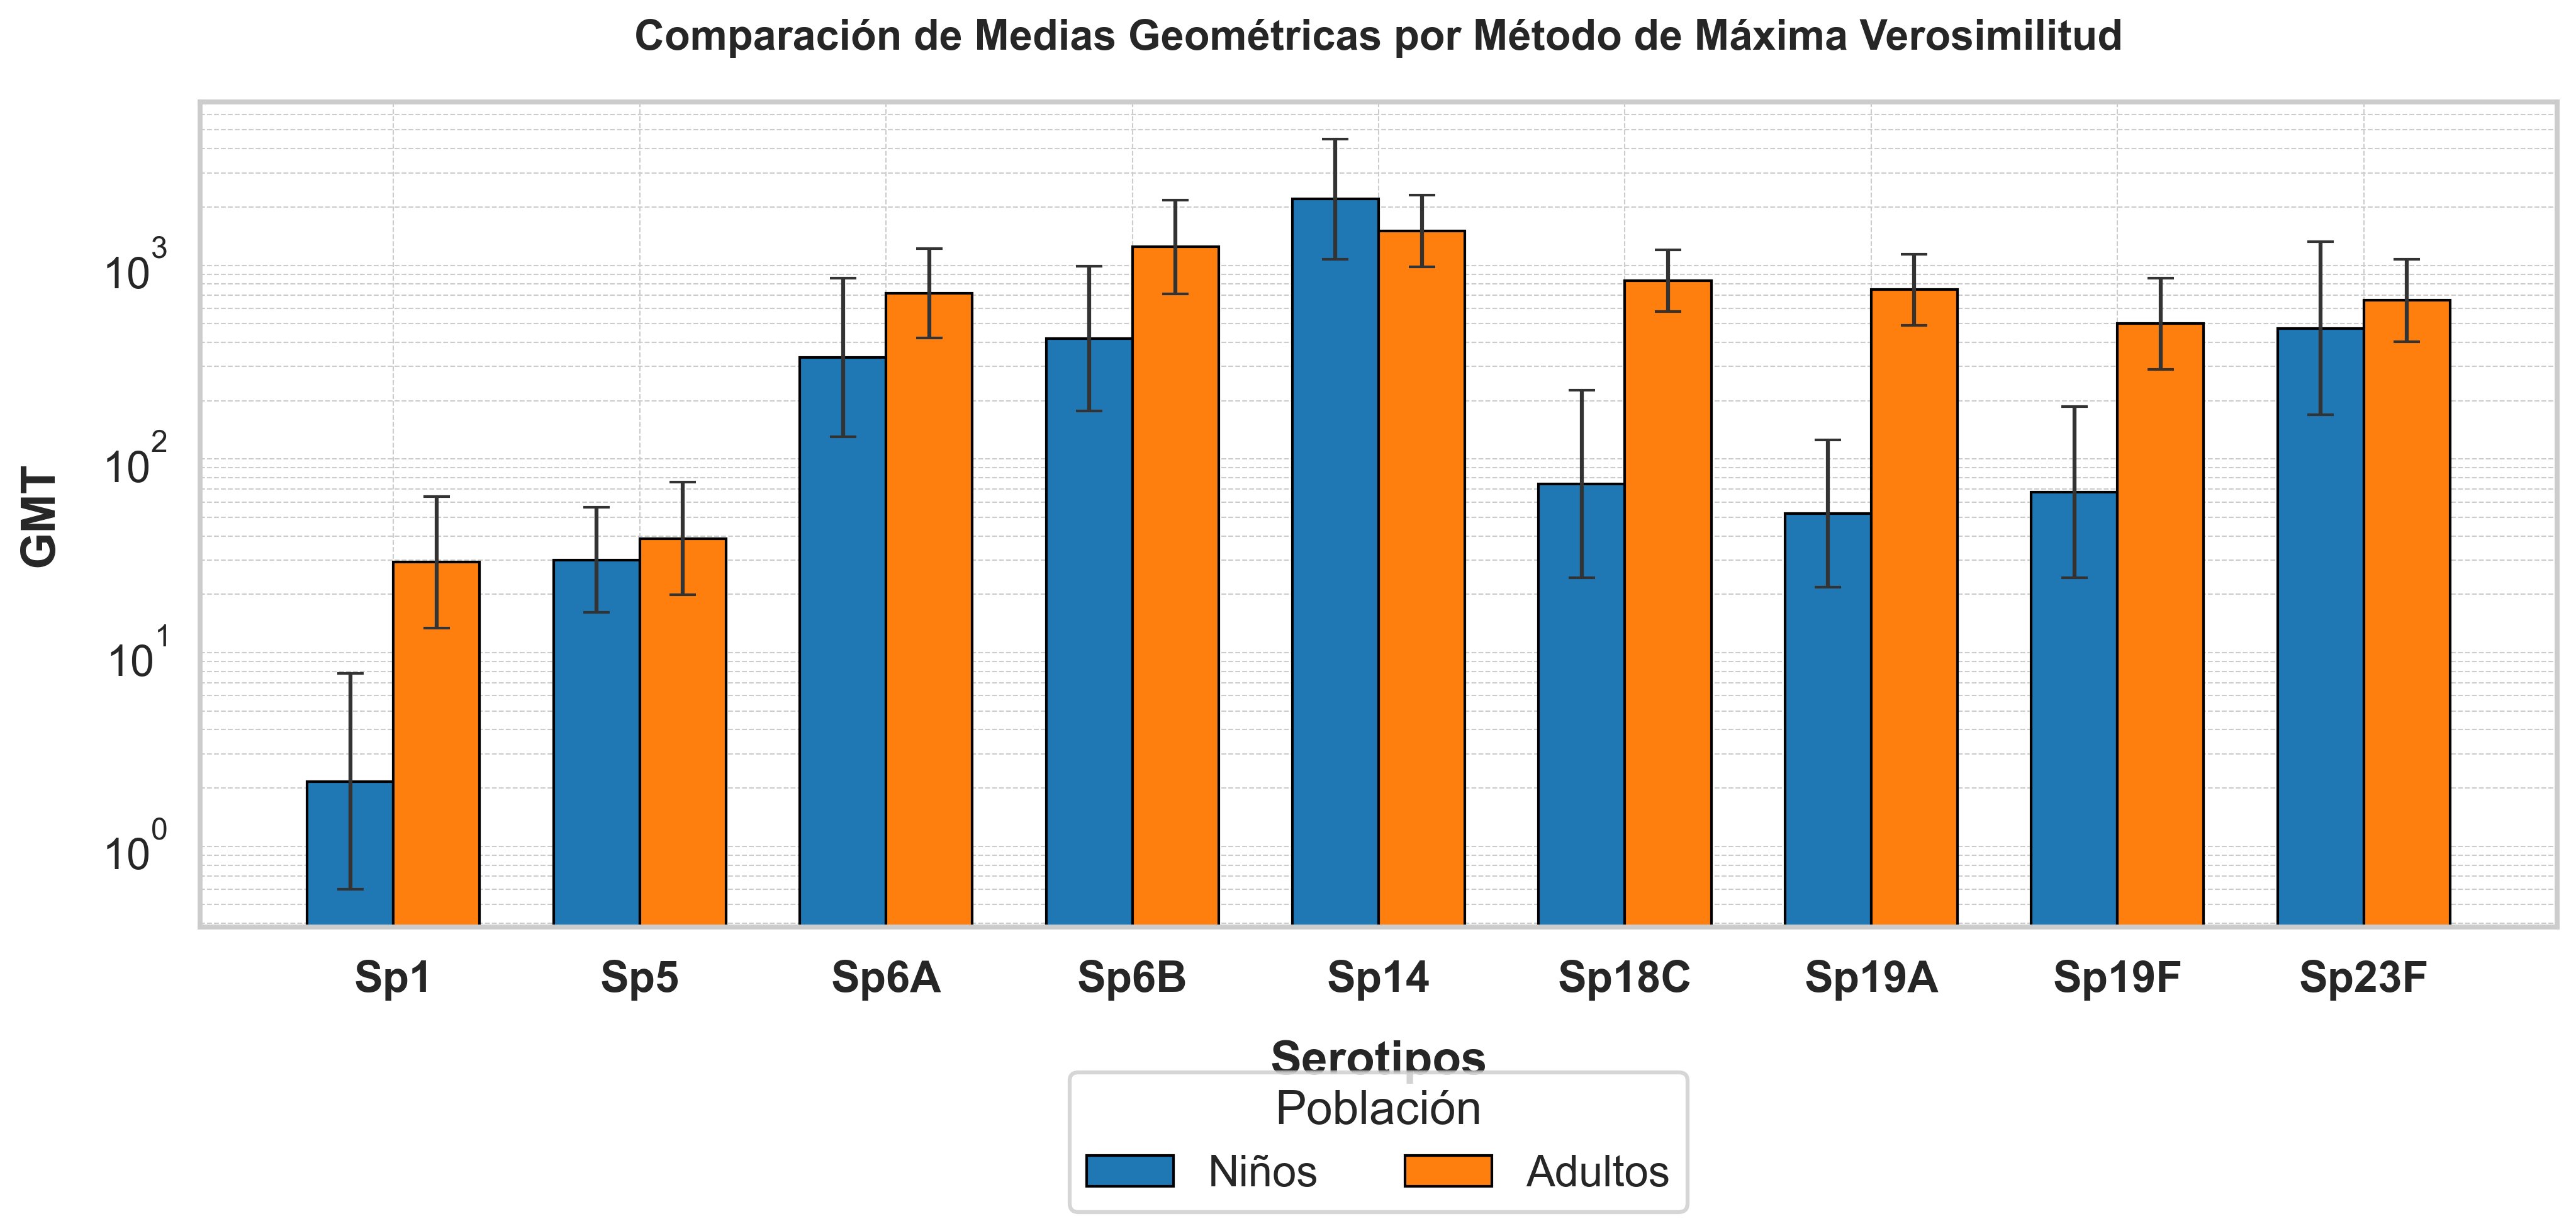
\includegraphics[width=1.0\textwidth]{Graphics/gmtm.png}
	\caption{Medias geométricas de los títulos utilizando el método de máxima verosimilitud.}
	\label{fig:gmt_graph2}
\end{figure}
\FloatBarrier

Por otra parte, los valores de las GMT difirieron considerablemente según el método estadístico utilizado. El método de máxima verosimilitud arrojó valores más bajos en comparación con el método de sustitución (Tabla \ref{tab:gmt_valores}).

\begin{table}[htbp]
	\centering
	\caption{Comparación de las Medias Geométricas de los Títulos (GMT) entre la población pediátrica y adulta según el método estadístico empleado.}
	\label{tab:gmt_valores}
	\begin{tabular}{lccccc}
		\toprule
		& \multicolumn{2}{c}{\textbf{Método de Sustitución}} & & \multicolumn{2}{c}{\textbf{Método MLE}} \\
		\cmidrule{2-3} \cmidrule{5-6}
		\textbf{Serotipo} & \textbf{Niños} & \textbf{Adultos} & & \textbf{Niños} & \textbf{Adultos} \\
		\midrule
		Sp1   & 13.49   & 45.89   & & 2.16   & 29.28   \\
		Sp5   & 42.54   & 48.08   & & 30.15  & 38.84   \\
		Sp6A  & 500.98  & 719.10  & & 334.20 & 715.48  \\
		Sp6B  & 581.55  & 1245.15 & & 418.76 & 1245.15 \\
		Sp14  & 2405.11 & 1499.53 & & 2194.62& 1504.39 \\
		Sp18C & 177.49  & 831.14  & & 74.10  & 831.14  \\
		Sp19A & 97.54   & 745.30  & & 52.26  & 749.21  \\
		Sp19F & 147.52  & 506.56  & & 67.36  & 498.97  \\
		Sp23F & 792.34  & 658.27  & & 472.34 & 658.27  \\
		\bottomrule
	\end{tabular}
\end{table}
\FloatBarrier

\section{Razón de medias geométricas y evaluación de no inferioridad}

Una vez estimadas las medias geométricas, se calcularon las razones de medias geométricas para cada serotipo, con sus respectivos intervalos de confianza del 95\%, para cada método. Luego de aplicar el contraste de hipótesis referente al estudio de inmunopuente, se demostró la no inferioridad para siete de los nueve serotipos analizados. Este resultado fue consistente en ambos métodos de análisis (Figura \ref{fig:forest_plot}).

\begin{figure}[ht]
	\centering
	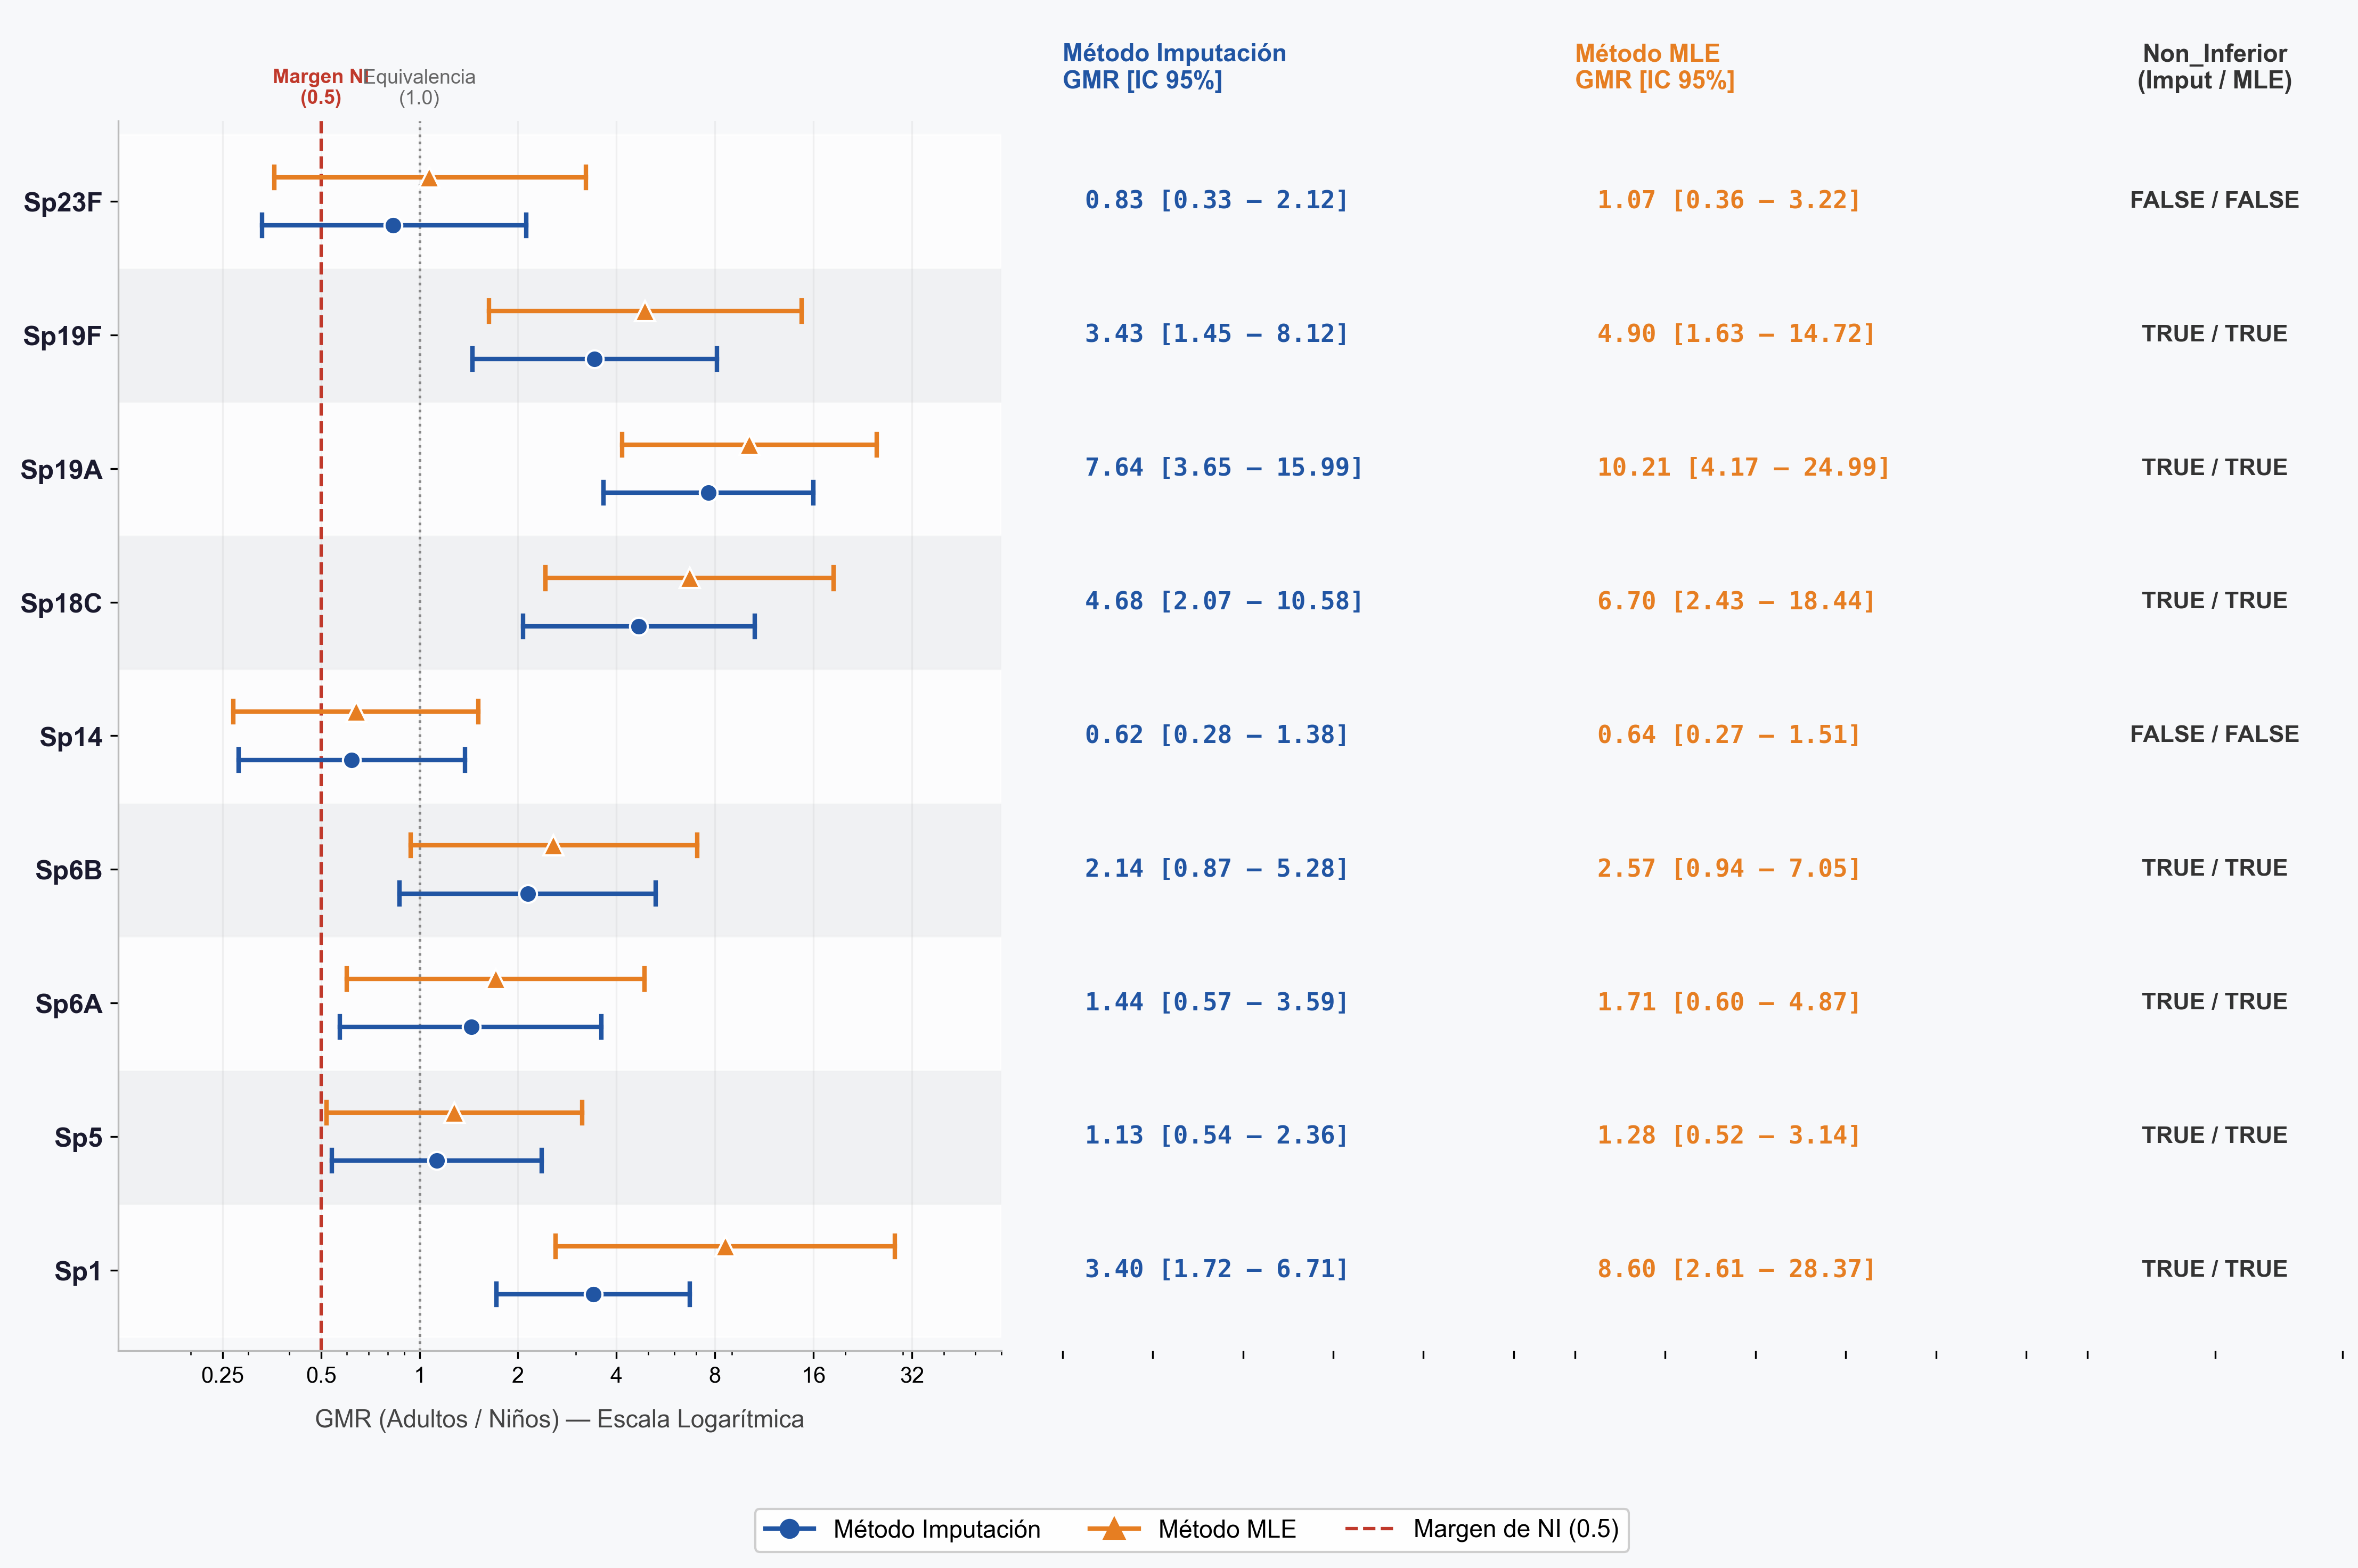
\includegraphics[width=1.0\textwidth]{Graphics/forest_plot_comparacion.png}
	\caption{No inferioridad de los 7 serotipos incluidos en Quimi-Vio 7 y los dos serotipos relacionados 6A y 19A.}
	\label{fig:forest_plot}
\end{figure}
\FloatBarrier

No se demostró la no inferioridad de los serotipos 14 y 23F. Aunque las estimaciones de sus GMR estuvieron por encima de 0.5, la alta variabilidad de los datos hizo que el límite inferior de sus intervalos de confianza cayera por debajo del margen de no inferioridad ($\delta = 0.5$).

Los intervalos de confianza obtenidos mediante el método de Wald mostraron una convergencia casi idéntica con aquellos estimados a través del perfil de verosimilitud. Esto confirma la simetría de la función de verosimilitud para las GMT y las GMR, y valida el uso de la aproximación de Wald como un método robusto y adecuado (véase Anexo \ref{tab:wald_vs_profile}).

Finalmente, el análisis de sensibilidad confirmó que la presencia de datos censurados no comprometió la determinación de no inferioridad en ninguno de los serotipos. No obstante, los serotipos con mayor porcentaje de censura presentaron medias geométricas más bajas e intervalos de confianza más amplios bajo el método MLE, comportamiento esperable dado que la amplitud de los intervalos está influenciada por la censura y por el tamaño muestral disponible en cada grupo \cite{pawitan2001all}.

(Tabla \ref {tab:resultados}).

\begin{table}[htbp]
	\centering
	\caption{Porcentajes de Censura y GMT con sus respectivos IC 95\% individuales por grupo etario (Método MLE).}
	\label{tab:resultados}
	\small
	\renewcommand{\arraystretch}{1.6} 
	\begin{tabular}{|l|c|c|c|c|c|c|}
		\hline
		& \multicolumn{3}{c|}{\textbf{Población Pediátrica (Niños)}} & \multicolumn{3}{c|}{\textbf{Población Adulta}} \\ \hline
		\textbf{Serotipo} & \textbf{N} & \textbf{Censura} & \textbf{GMT [IC 95\%]} & \textbf{N} & \textbf{Censura} & \textbf{GMT [IC 95\%]} \\ \hline
		Sp1   & 81 & 66.7\% & 2.16 [0.60, 7.80]       & 63 & 38.1\% & 29.28 [13.37, 64.10]   \\ \hline
		Sp5   & 80 & 35.0\% & 30.15 [16.12, 56.37]    & 63 & 23.8\% & 38.84 [19.89, 75.84]   \\ \hline
		Sp6A  & 75 & 28.0\% & 334.20 [129.96, 859.47] & 63 & 6.3\%  & 715.48 [421.30, 1215.06] \\ \hline
		Sp6B  & 81 & 25.9\% & 418.76 [177.19, 989.67] & 64 & 0.0\%  & 1245.15 [712.95, 2174.63]\\ \hline
		Sp14  & 82 & 14.6\% & 2194.62 [1077.46, 4470.09] & 64 & 1.6\%  & 1504.39 [984.47, 2298.89]\\ \hline
		Sp18C & 78 & 39.7\% & 74.10 [24.31, 225.88]   & 62 & 0.0\%  & 831.14 [576.17, 1198.93] \\ \hline
		Sp19A & 81 & 38.3\% & 52.26 [21.71, 125.83]   & 63 & 3.2\%  & 749.21 [491.01, 1143.19] \\ \hline
		Sp19F & 82 & 39.0\% & 67.36 [24.39, 186.00]   & 61 & 11.5\% & 498.97 [289.23, 860.80]  \\ \hline
		Sp23F & 83 & 28.9\% & 472.34 [168.73, 1322.26] & 64 & 0.0\%  & 658.27 [404.30, 1071.78] \\ \hline
	\end{tabular}
\end{table}
\FloatBarrier

\begin{figure}[ht]
	\centering
	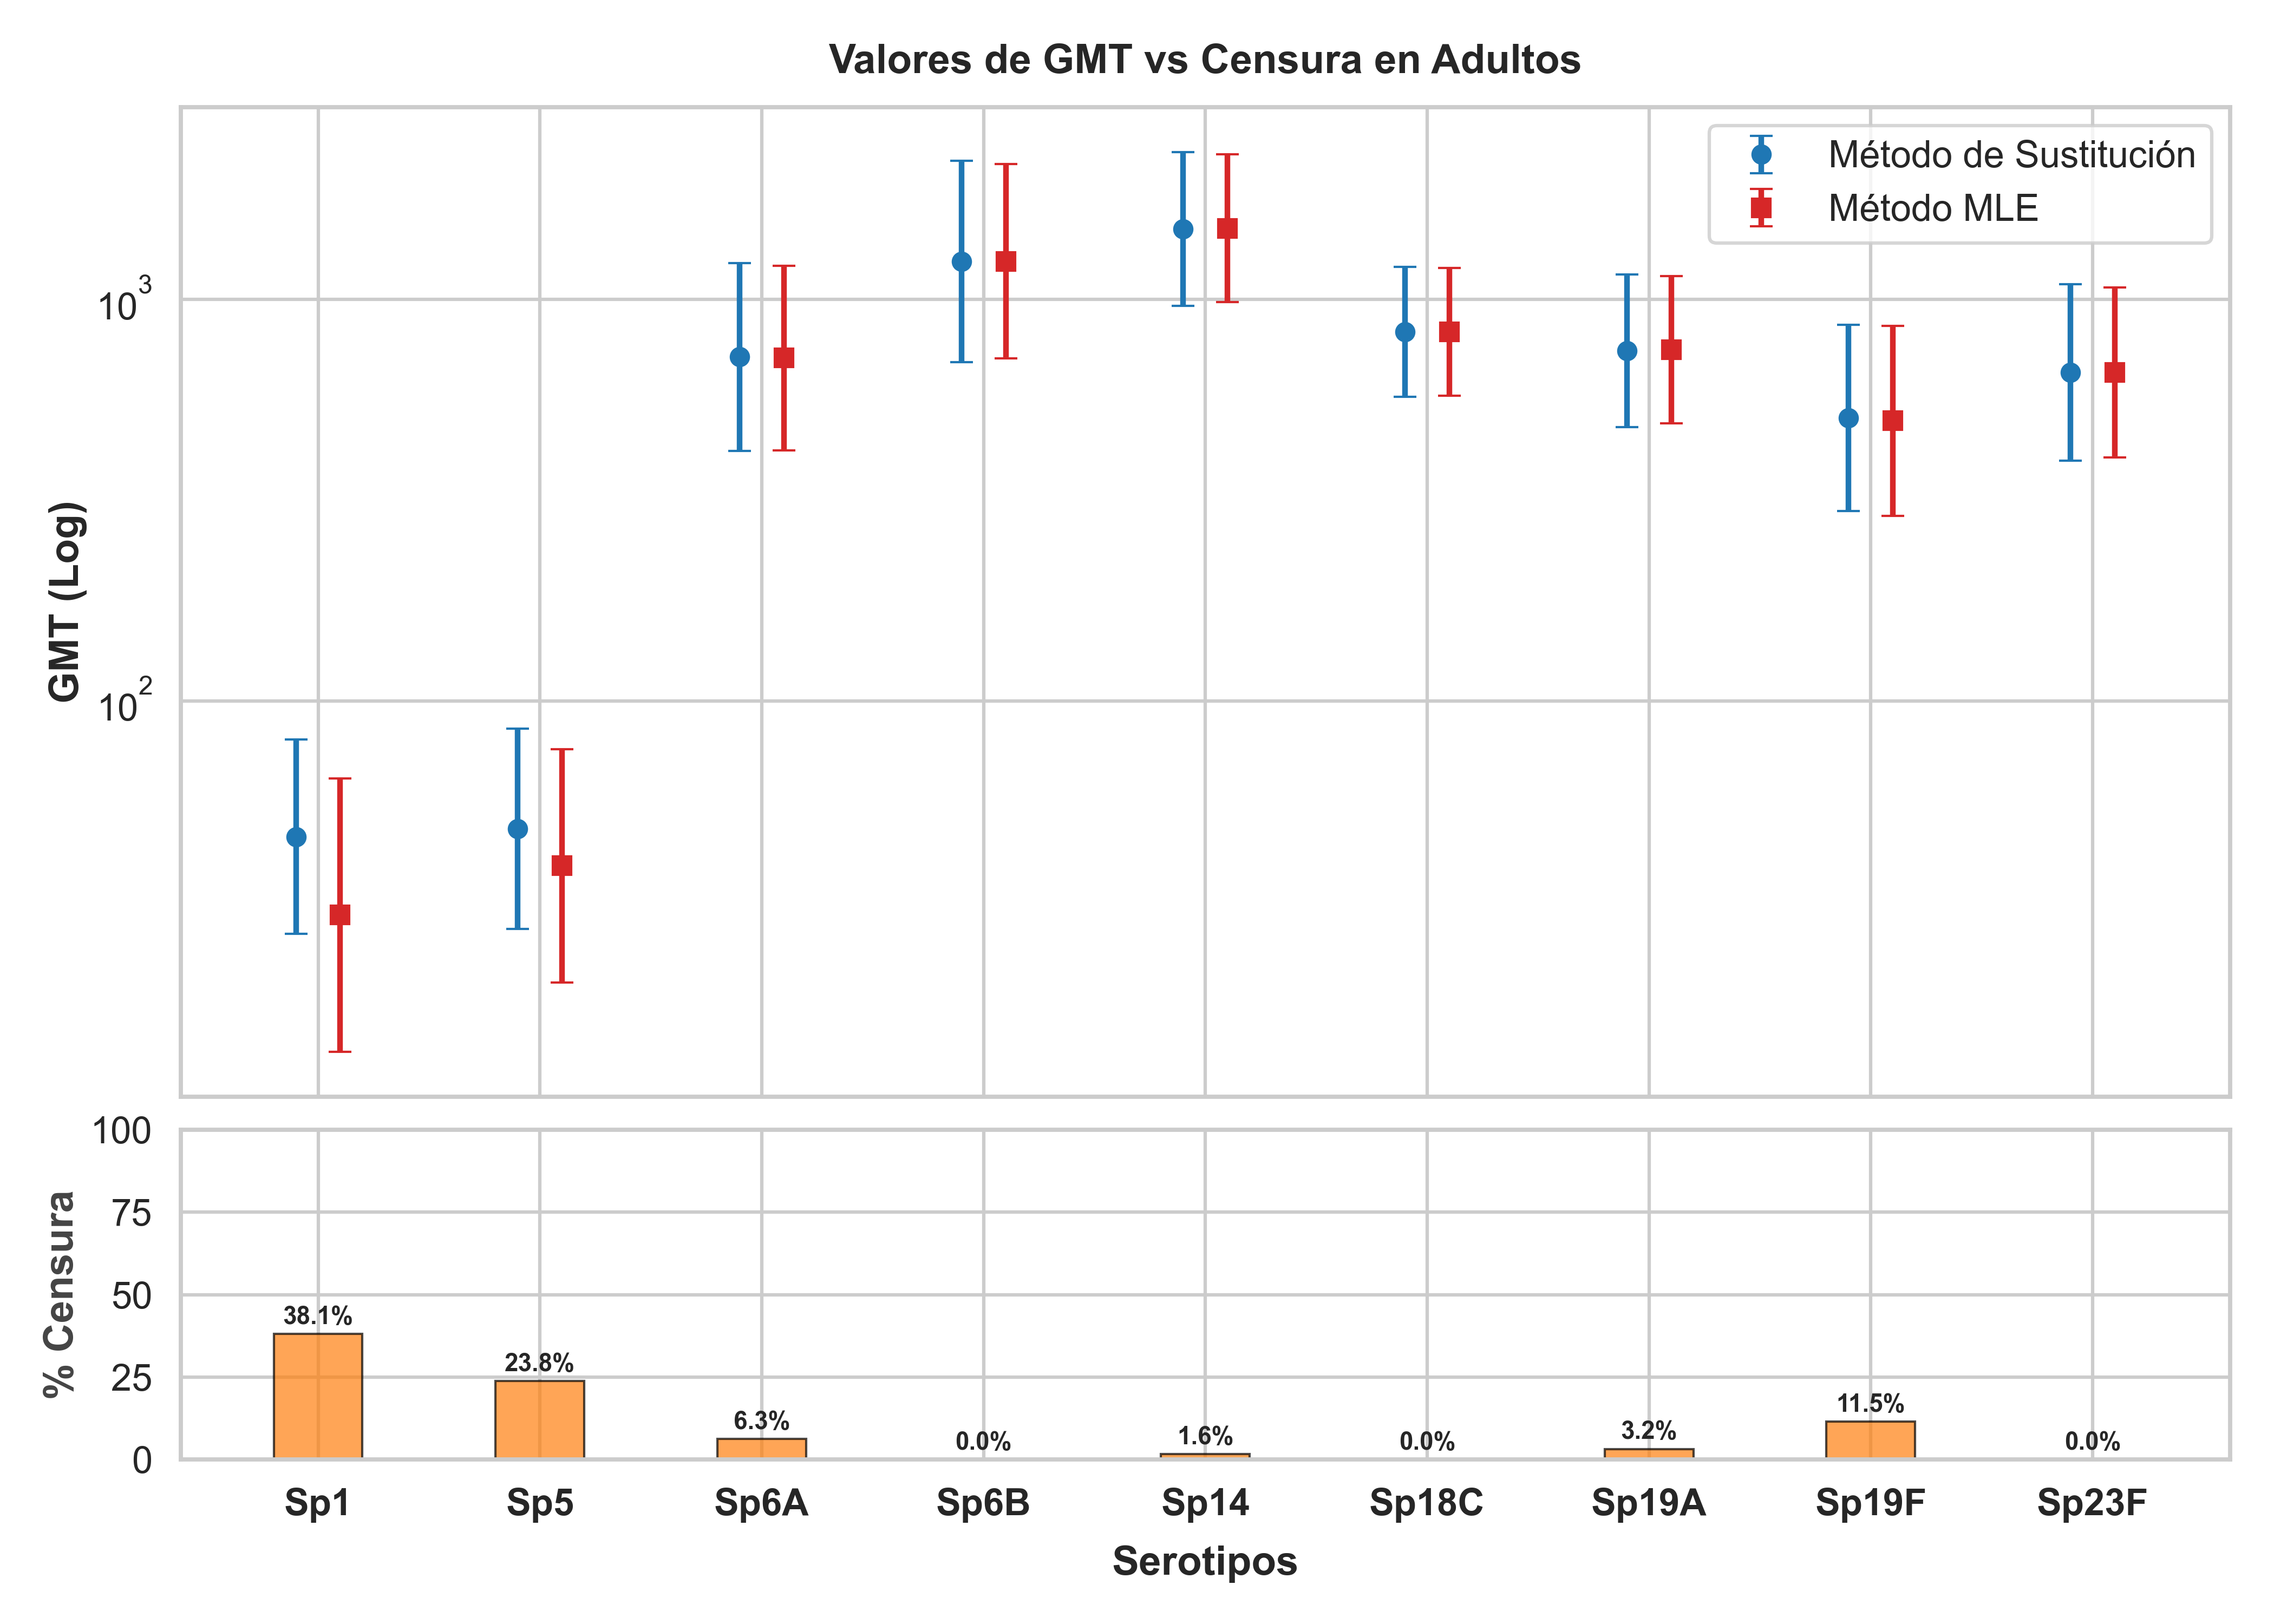
\includegraphics[width=1.0\textwidth]{Graphics/GMT_vs_Censura_Adultos.png}
	\caption{Comparación de los valores de medias geométricas para ambos métodos teniendo en cuenta la censura por serotipo en adultos.}
	\label{fig:gmt_adultos}
\end{figure}
\FloatBarrier


\begin{figure}[ht]
	\centering
	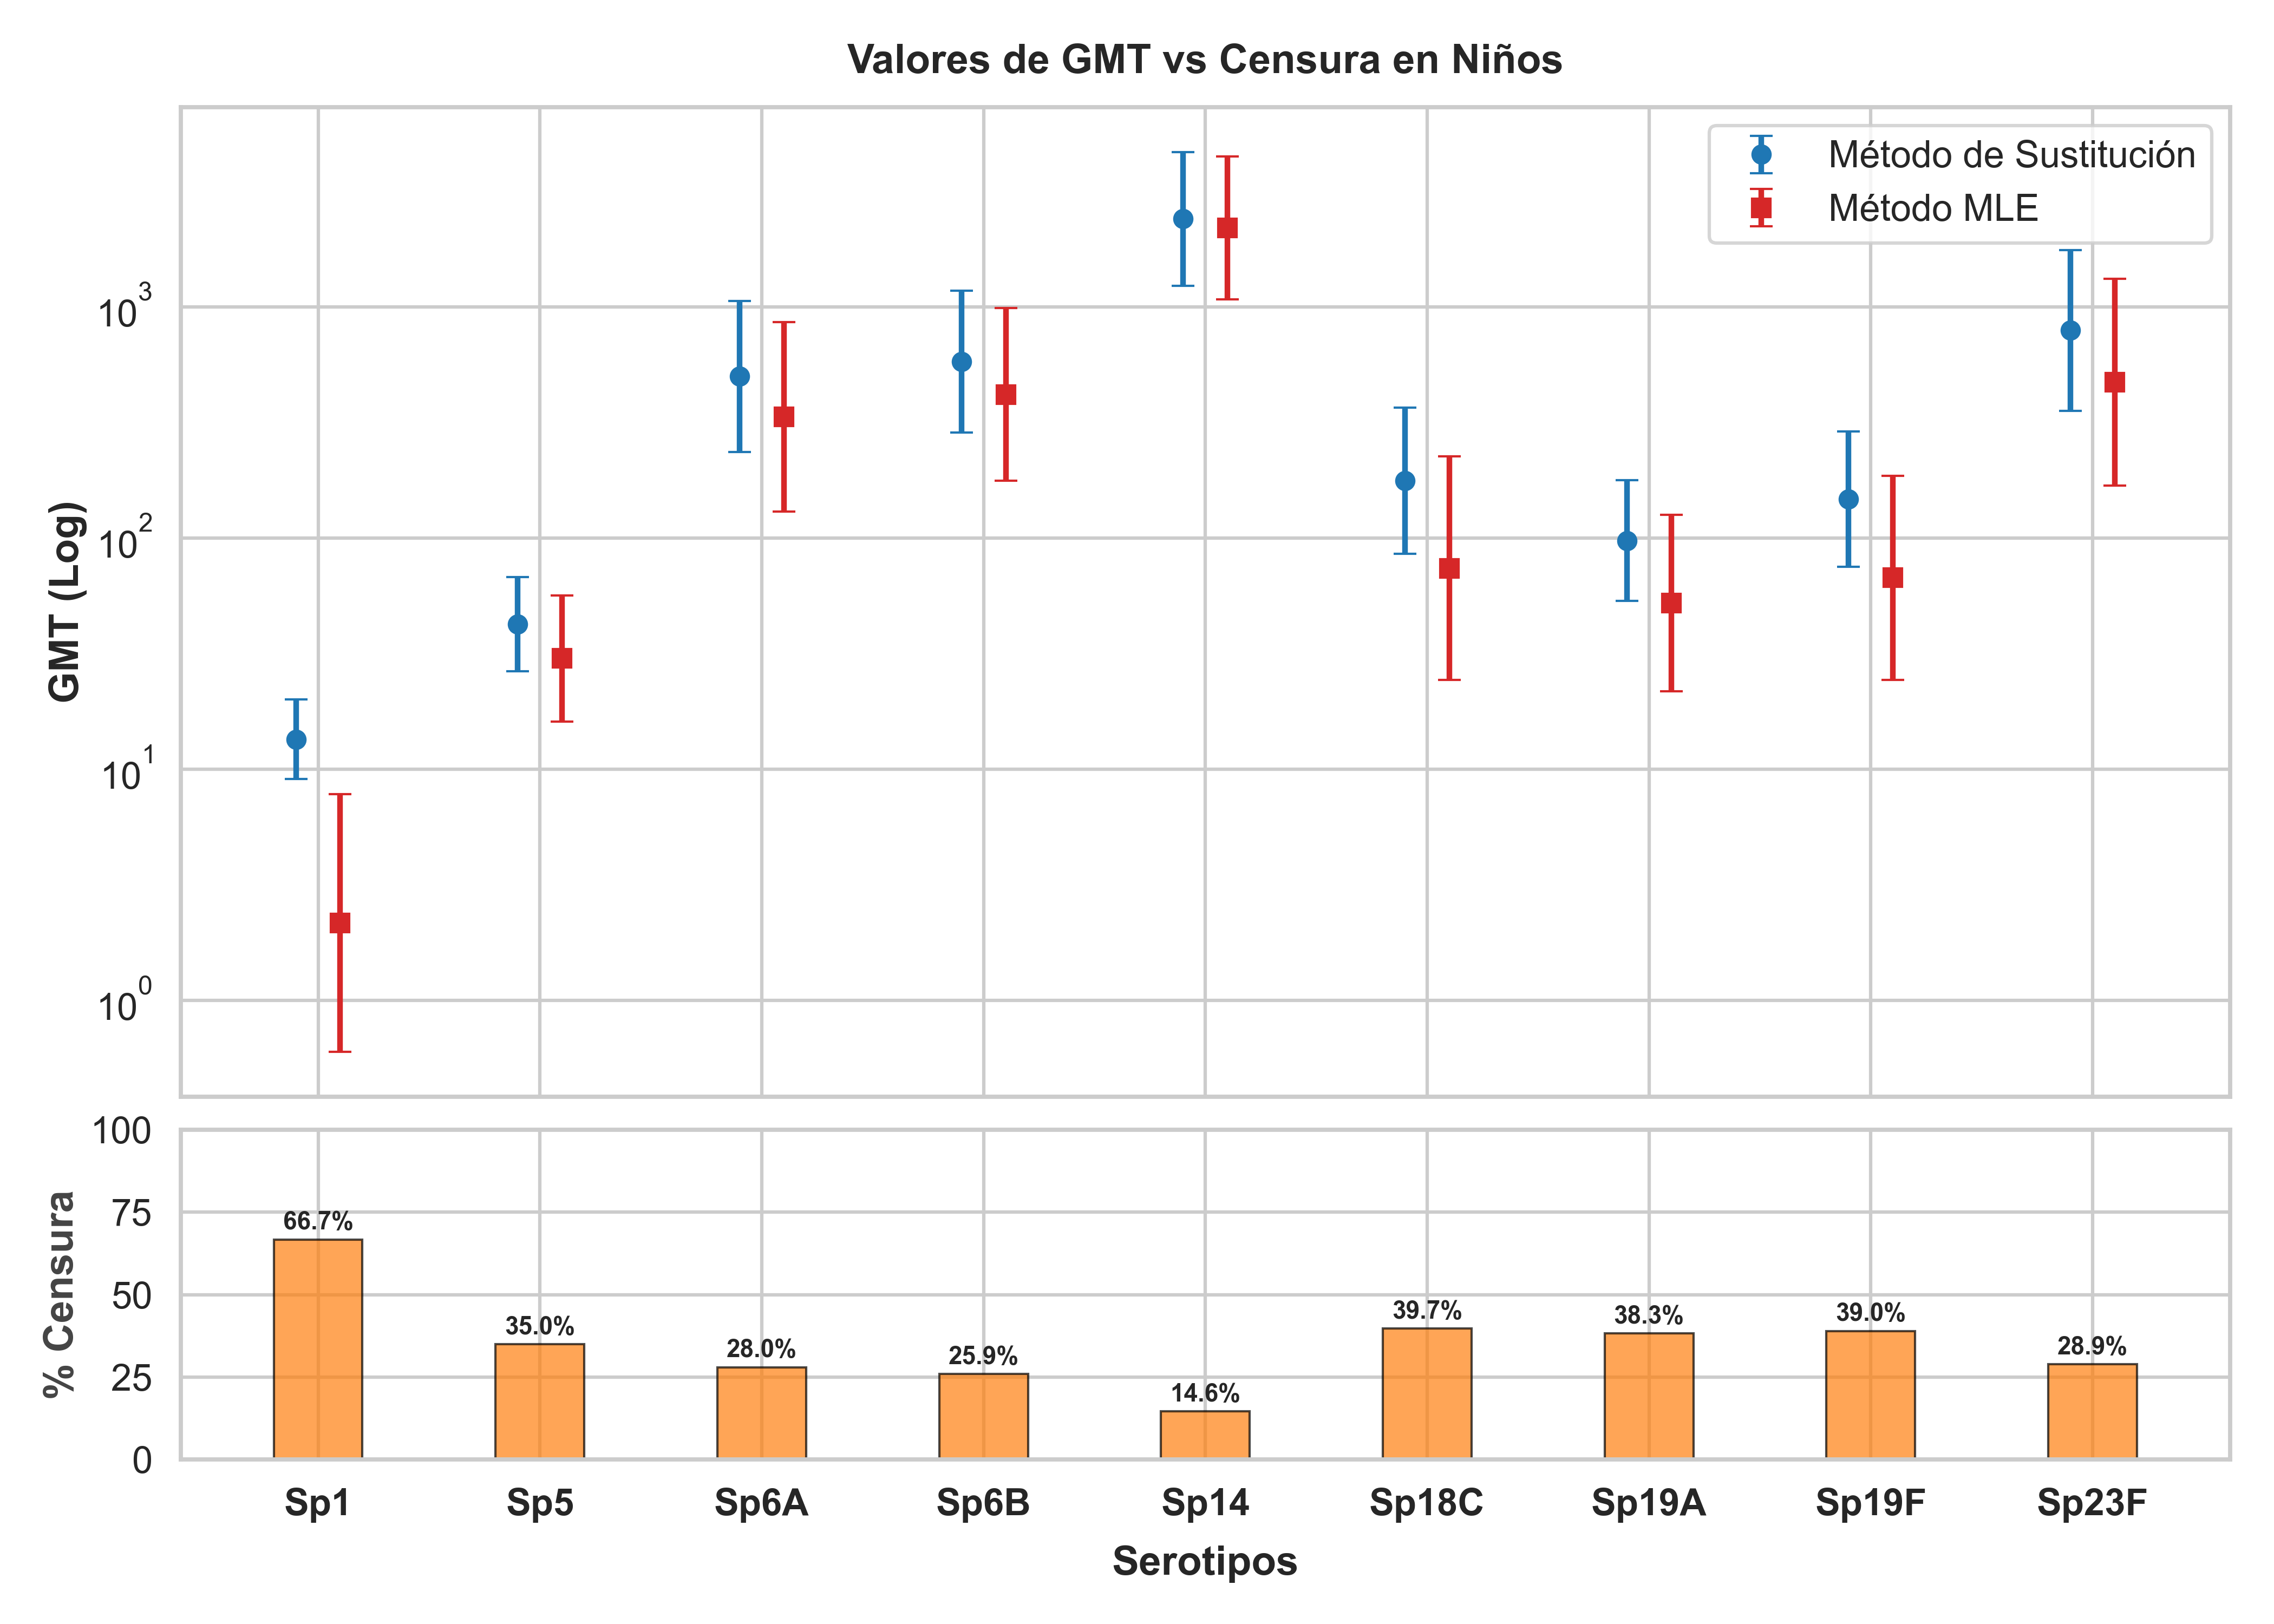
\includegraphics[width=1.0\textwidth]{Graphics/GMT_vs_Censura_Ninnos.png}
	\caption{Comparación de los valores de medias geométricas para ambos métodos teniendo en cuenta la censura por serotipo en niños.}
	\label{fig:gmt_ninnos}
\end{figure}
\FloatBarrier